% !BIB program = biber


\documentclass[doc]{apa6}

\usepackage[utf8]{inputenc}
\usepackage[american]{babel}
\usepackage{todonotes}
\usepackage{csquotes}
\usepackage[style=apa,sortcites=true,sorting=nyt,backend=biber]{biblatex}
\DeclareLanguageMapping{american}{american-apa}
\usepackage{adjustbox}
%\addbibresource{bibliography.bib}
\addbibresource{zot3.bib}
\usepackage{boxedminipage}
\usepackage[toc,page]{appendix}
\usepackage{hyperref}
\usepackage{color}
\usepackage[normalem]{ulem}

% ---------- watermark -----------
\usepackage[firstpage]{draftwatermark}
\SetWatermarkAngle{0}
\SetWatermarkFontSize{0.25cm}
\SetWatermarkVerCenter{1cm}
\SetWatermarkLightness{0.5}
\SetWatermarkHorCenter{14cm}
\SetWatermarkText{\shortstack[l]{
Kennedy, L. A., Navarro, D. J., Perfors, A. and Briggs N. (2017). Not every \\
credible interval is credible: Evaluating robustness in the presence of \\
contamination in Bayesian data analysis. Behavior Research Methods, 49, \\
2219–2234. https://doi.org/10.3758/s13428-017-0854-1}}
\SetWatermarkScale{1}
% -------------------------------



\title{Not every credible interval is credible: Evaluating robustness in the presence of contamination in Bayesian data analysis}
\shorttitle{Robust credible intervals}

\fourauthors{\normalsize Lauren A. Kennedy}{\normalsize Danielle J. Navarro}{\normalsize Amy Perfors}{\normalsize Nancy Briggs}
\fouraffiliations{School of Psychology\\University of Adelaide}{School of Psychology\\University of New South Wales}{School of Psychology\\University of Adelaide}{Mark Wainwright Analytical Centre\\University of New South Wales}

    \abstract{As Bayesian methods become more popular among behavioral scientists, they will inevitably be applied in situations that violate the assumptions underpinning typical models used to guide statistical inference. With this in mind, it is important to know something about how robust Bayesian methods are to the violation of those assumptions. In this paper we focus on the problem of {\it contaminated} data (such as data with outliers or conflicts present), with specific application to the problem of estimating a credible interval for the population mean. We evaluate     five   Bayesian methods for contructing a credible interval, using toy examples to illustrate the qualitative behavior of different approaches in the presence of contaminants, and an extensive simulation study to quantify the robustness of each method. We find that the ``default'' normal model used in most Bayesian data analyses is not robust, and that approaches based on the Bayesian bootstrap are only robust in limited circumstances.   A   simple parametric model based on Tukey's ``contaminated normal model''     and a model based on the t-distribution were   markedly more robust.   However, the contaminated normal model had the added benefit of estimating which data points were discounted as outliers and which were not.   }

\keywords{Bayesian data analysis, robust methods, contaminated data}

\begin{document}

\maketitle

Data analysis plays a central role in scientific discovery, helping researchers organize and interpret the results of experimental and observational studies. In the majority of cases, researchers conduct data analyses with the help of ``default'' models that are broadly applicable to a wide range of scientific problems, rather than attempt the more arduous (and often unrealistic) task of developing a task specific model for each problem. As a consequence of this pragmatic behavior by scientists, it is important to verify whether these default models behave in a sensible way when applied to real data that may not satisfy the assumptions built into the model. Much of the applied statistics literature has this character \parencite{bamnett1994outliers,wilcox_introduction_2012,hoaglin2011exploring}.

Because the world is complex and data are limited, it is generally recognized that it is never possible to build a model that is detailed enough to capture everything of interest in a particular data analysis problem: it is for this reason that statisticians often remark that ``all models are wrong'' \parencite[e.g.,][]{box_science_1976}.   This is also why   examining the performance of models when their assumptions are violated (i.e., when the model is {\it misspecified}) is critically important for ensuring sound scientific practice.   Following the advice of \textcite{box_science_1976}, our goal here is to determine which models are most useful when their assumptions are violated.

With this in mind, it is useful to consider the rise of Bayesian data analysis in behavioral statistics. Orthodox statistical inference begins from the frequentist premise, which assumes that the word ``probability'' describes the results of an {\it aleatory} process: when a repeatable event such as the flip of a coin is repeated sufficiently many times, in the long run the proportions of cases converge to a specific number (e.g., 50\% of coin flips come up heads). The vast majority of analyses in the psychological literature rely on orthodox statistical theory: when reporting confidence intervals and $p$-values, for instance, one is relying on frequentist methods.

Unlike the orthodox approach, the Bayesian view does not interpret probability in aleatory terms. Instead, the Bayesian approach begins from an {\it epistemic} assumption, and interprets the word ``probability'' as the degree of belief that a       reasoner should place in an particular proposition. Over the last few decades, the Bayesian approach has become increasingly popular, with many researchers choosing to report Bayes factors rather than $p$-values and credible intervals instead of confidence intervals. In part this shift has been driven by the well-documented failures of orthodox methods \parencite{wagenmakers_practical_2007}, and in part by the fact that there are now several easily accessible tools that provide default Bayesian solutions to common data analysis problems \parencites[  for a default t-distribution model see][  online version;  \url{http://www.sumsar.net/best_online/}]{BESTpackage}. For instance, the development of the BayesFactor package in R \parencite{Morey_2015_BF} and its easy accessibility through user friendly software such as JASP \parencite{jasp_2016} has allowed widespread adoption of Bayesian methods that were once available only to specialists. In our view this mainstreaming of Bayesian inference is greatly to be desired, but it carries new problems for Bayesian statisticians to consider.   In particular, when Bayesian analyses were more inaccessible, that meant that the only people who implemented Bayesian statistics were technically sophisticated enough not to misuse them; as they become more mainstream -- which is a good thing! -- it does mean that they are also more likely to be applied inappropriately or misused.

What challenges are these? In an ideal world, the answer would be ``none at all'': every researcher would consider the particular constraints imposed by their research problem, work out what those constraints imply about the statistical model to be used, {construct the priors that best express the knowledge that the researcher possesses, implement that model, and then report the posterior distributions that result once the data are observed. In the real world, of course, this is not so much a polite fiction as it is a statistician's fantasy. In our experience researchers (sometimes) do not have rich enough knowledge of the problem or (very often) lack the many years of statistical training required do anything other than rely on default methods.

As default Bayesian tools become mainstream, they will increasingly be used in situations that violate their assumptions. As such, it is critical to consider how well default Bayesian methods perform when they are misspecified, and to consider whether different defaults are required if performance is especially poor with respect to common problems. There are a many different situations in which model misspecification becomes a concern: in this paper we focus on the problem of \textit{contaminated data}. Contaminated data problems arise when a researcher's observations are composed not just of data that reflects the question of interest, but also data reflecting some other generating process.


\subsection{The problem of contaminated data}

We frame the problem of contaminated data in terms of one of the simplest estimation problems in statistics: using observed data $X=(x_1,\ldots,x_n)$ to construct an interval estimate for a population mean. Very typically we might assume that the observed data are drawn from a normal distribution with unknown mean $\mu$ and standard deviation $\sigma$. In most cases the quantity of interest is the unknown mean $\mu$. With the help of this model, an orthodox statistician might construct a confidence interval that is designed to ensure that $\mu$ falls within the interval for 95\% of cases, or a Bayesian statistician might construct a credible interval and claim that there is a 95\% chance that the true mean falls within the range. Regardless of whether one is Bayesian or frequentist, the analyses that empirical scientists usually rely upon assume that every observation $X$ has been sampled from the relevant population distribution.

In many -- perhaps most -- real world inference problems facing psychological researchers, this assumption is untenable. Sometimes participants press buttons randomly in the hope of leaving the study early, sometimes people answer the wrong question, sometimes a legitimate response is miscoded in the data. As a consequence, most data sets end up with some unknown proportion of {\it contaminants}; observations that arise from some other unknown process and are not informative about the population parameters of interest to researchers. To the extent that one's statistical inferences are driven by contaminants, researchers run the risk of drawing the wrong conclusions from experimental data.

The difficulties posed by contaminants are well known both to empirical scientists and to statisticians, and the issue is very frequently covered in introductory research methods classes. Researchers typically use exclusion criteria to try to identify contaminants and remove them from data sets. Similarly, statisticians have developed a variety of {\it robust} methods that are designed to produce sensible inferences even when contaminants are present, from both a Bayesian \parencite{wang_general_2015,berger_overview_1994} and frequentist perspective \parencite{huber_robust_1964,huber_robust_2009}. In this paper we approach the problem from a Bayesian perspective.

To what extent does contamination present a problem for Bayesian data analysts? One possibility is that all Bayesian methods are robust to contamination simply by virtue of being Bayesian. This may seem somewhat implausible to an expert reader -- and we imagine that statisticians would recognize this as the strawman hypothesis that it is -- but Bayesian approaches often seem so desirable that experimental researchers could certainly be forgiven for thinking that this is a serious possibility. With this in mind, in the next section we will focus on relatively simple Bayesian models that can easily be applied to typical experimental data in the behavioral sciences, and investigate the differences between them when contaminants are present.

\section{Four ways to get five posteriors}

We focus on the relatively simple situation in which a researcher is presented with a sample of $n$ continuous-valued  univariate observations $X=(x_1,\ldots,x_n)$, and the goal is to construct an interval that captures the researcher's uncertainty about the population mean. Although this situation is somewhat limited in scope, it corresponds to a very common problem in psychological research, since it is quite typical for researchers to examine and report means and confidence intervals (or the Bayesian equivalent).  In this section we describe     five   different     methods \footnote{Code implementing the models can be found online at \url{https://github.com/lauken13/Robust-Intervals}} that a Bayesian researcher might use to construct a   highest density   credible interval when presented with this inference problem: the {\it normal} model, the {\it contaminated normal} model,    the {\it $t$ distribution model},   and two versions of the {\it Bayesian bootstrap} method.\footnote{In our initial investigations we also considered two frequentist methods for estimating confidence intervals, one of which was the Student's $t$ interval and the other of which was the 20 \% percentile-$t$ trimmed bootstrap. Not surprisingly the overall behavior of the Student's $t$ interval was roughly similar to that of the Bayesian normal model, and the frequentist trimmed bootstrap was somewhat similar to the Bayesian trimmed mean bootstrap. However, given that the behavior of the frequentist methods is well-documented elsewhere in the literature and that our goal in this paper is not to revisit the ``Bayesians versus frequentist'' debate yet again, we decided to omit the frequentist methods.}


\subsection{The normal model}

The first model we consider is a ``default'' normal model that makes no attempt to address the problem of contaminants. As shown in Figure~\ref{graphicalmodels}a this model assumes that all observations are sampled independently from a normal distribution with unknown mean $\mu$ and unknown standard deviation $\sigma$. Because these parameters are unknown, the researcher specifies priors that describe their pre-existing state of knowledge. We restrict ourselves to the grossly typical situation in which the researcher has very little prior knowledge about the parameters, and specifies diffuse priors over $\mu$ and $\sigma$. To formalize this, we adopt a prior in which $\mu$ is drawn from a Normal(0,100) distribution and the precision of the data (i.e., $1/\sigma^2$) is drawn from a Gamma(.0001, .0001) distribution, but other variations are possible. Following typical practice in the Bayesian data analysis literature we implemented this model using JAGS, though given the simplicity of the model almost any software package could be used. The normal model appears in various guises in the Bayesian data analysis literature, for example the basic Bayesian t-test \parencite{wetzels2009quantify}, Bayesian ANOVA \parencite{rouder2012default}, and many other custom models \parencite{lee2014bayesian}.


\begin{figure}[t]
    \centering
    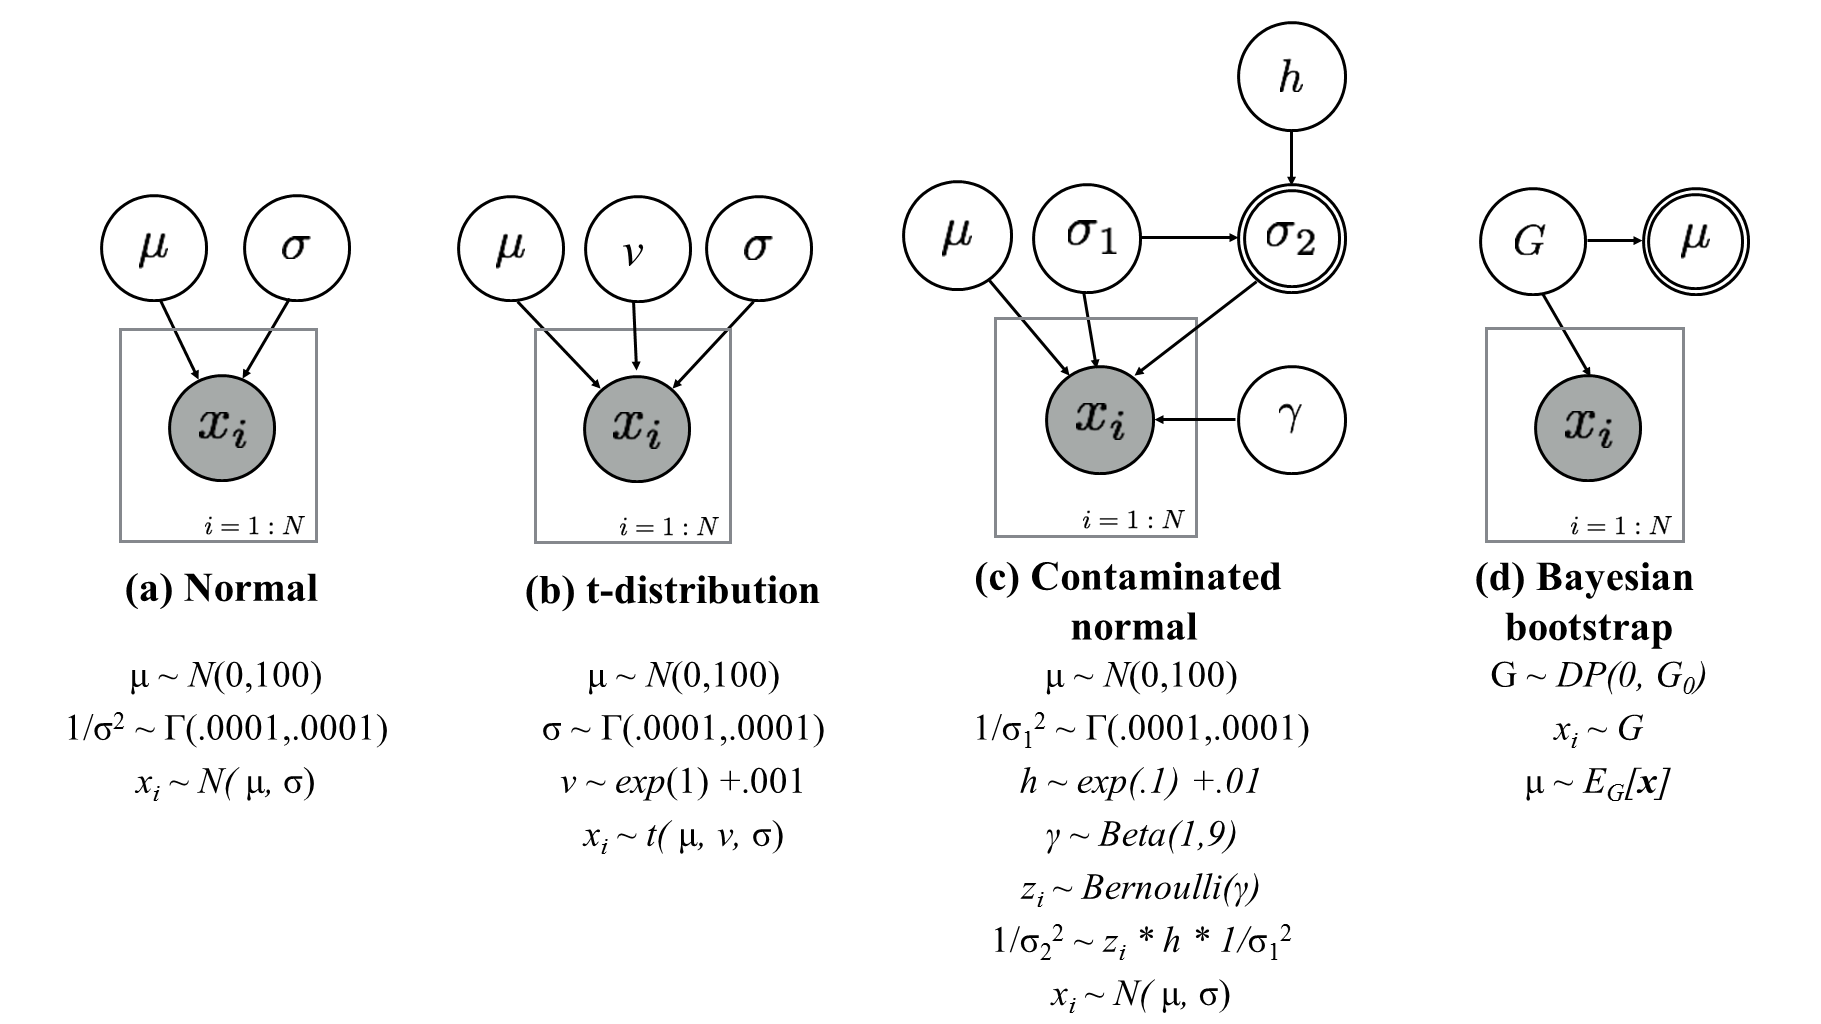
\includegraphics[width=15cm]{graphicalmodels.png} \vspace*{6pt}
    \caption{Graphical models for the usual normal model (panel a),  the t-distribution model (panel b),   the contaminated normal model (panel    c ), and the statistical model underpinning the Bayesian bootstrap procedure (panel       d).   Beneath the graphical models we have included prior and relational information about each node. Wherever sensible we have endeavoured to keep the priors for similar parameters similar across the models.}
    \label{graphicalmodels}
\end{figure}


\subsection{The t-distribution model}
\textcite{andrade2011bayesian} and \textcite{kruschke2013bayesian} suggest a convenient alternative to the normal model. These authors take the view that the normal distribution is very sensitive to outliers, and note that this sensitivity can be reduced if the data are assumed to arise from a distribution with heavier tails. With that in mind, they suggest that the t-distribution is a convenient heavy tailed distribution that only adds one additional free parameter (degrees of freedom) when compared to the normal model. Theoretically this distribution is created from a mixture of normals with expected value $\mu$ and a precision drawn from $Gamma(df/2, scale^2*df/2)$. The full model is depicted graphically in Figure~\ref{graphicalmodels}b.

In order to allow for direct comparison across models we chose to use the same prior for $\mu$ and precision parameters as the normal model. For the degrees of freedom we use an exponential prior as recommended by \textcite{kruschke2013bayesian}. In order to avoid increased flexibility due to hyper-parameters, we use $\exp(1)$ as the prior, which is relatively conservative in the amount of variation in the standard deviations of the normals in the mixture.

This model construction promises to be robust when faced with outliers. Each datum observed can be thought of as a draw from a normal distribution with the same mean as other data in the sample, but with a precision that is wider or narrower as dictated by its relationship to the rest of the data (i.e. a more extreme point would be drawn from a normal with lower precision and hence higher variance). Whilst theoretically this is true, the data as a whole is fit to a t-distribution with parameters $\mu$, $\sigma$ and $\nu$ (degrees of freedom). This final parameter, $\nu$, provides the only indication to the amount of data that is discounted as outliers or contaminants. The exact relationship, however, is not clear. Certainly it does not give an estimate of the proportion of data that are discounted, nor the degree to which they are discounted. With this in mind, we propose an alternative model that does allow the user some notion of the proportion and extremity of the contamination.


\subsection{The contaminated normal model}

As an alternative to the normal and t-distribution models, we propose the {\it contaminated normal} model \parencite[e.g.,][]{tukey_survey_1960}. Although this model requires an additional number of free parameters, we argue that it is easier overall to interpret. The contaminated normal is a very simple mixture model in which the target distribution is again a normal distribution with unknown mean $\mu$ and standard deviation $\sigma_1$, as per the usual normal model. However, some unknown proportion of the observations $\gamma$ are drawn from a contaminant distribution that again has mean $\mu$ but has a different (generally larger) standard deviation $\sigma_2$. The standard deviation of the contaminants is governed by the scale parameter $h$, such that $\sigma_2 = h \times \sigma_1$. The contaminated normal model is depicted graphically in Figure~\ref{graphicalmodels}  c .

In our applications we assume that the contaminant proportion $\gamma$ is drawn from a Beta(1,9) distribution, reflecting a  somewhat conservative expectation that 10\% of the data are contaminants. Similarly, we assume that $h$ is drawn from an Exponential(.1) distribution, implying that on average the contaminant distribution will be 10 times as wide as the target distribution.   The model enumerates the probability each datum is a contaminant and the overall proportion of contamination.

Clearly, the contaminated normal model is not intended to serve as a literal model for how contamination processes play out in psychological data. In real life there are very few phenomena of interest to behavioral researchers that are precisely normally distributed, and there is no reason to think that contaminant distributions are any more likely to be normal either. However, in much the same way that researchers treat normality as a sensible first approximation when constructing models for a phenomenon of interest, we propose that normality makes sense as a first approximation to contaminant processes too. Our goal is not to have a realistic generative model for every psychological experiment (which seems impossible) but rather to construct a minimal, sensible account that has the potential to detect the most misleading contaminants and prevent them from having a disproportionately large effect on the inferences about the target.

To our knowledge the contaminated normal model has not previously been considered as a general purpose tool in psychological data analysis, but the principles upon which it is based are fairly standard. For example, the idea of explicitly building a high-variance ``contaminant distribution'' into the model is a relatively standard approach in cognitive modelling \parencite[e.g.,][]{zeigenfuse_general_2010,ratcliff_estimating_2002}. Similarly, the overall effect of adding the contaminant distribution is to create a ``heavy tailed'' model for the observed data, consistent with standard advice in the Bayesian robust statistics literature \parencite[e.g.,][]{berger_overview_1994}. Given the simplicity of the idea and its alignment with existing approaches in the literature, the contaminated normal model seems a sensible way to construct a default model for contaminated data.


\subsection{The Bayesian bootstrap}

In the contaminated normal model, the central idea is to model contaminants with the help of an explicit, parameterized contaminant distribution. The model is very much a parametric model, making strong assumptions about the shape of the target distribution and the shape of the contaminant distribution. An alternative approach is to consider nonparametric methods in which the researcher avoids relying on any strong assumption about distributional shape. This approach is very common in frequentist analyses: when presented with unusual data, a typical orthodox solution is to use bootstrapping \parencite{efron1994introduction} to construct confidence intervals \parencite{hall1988symmetric,efron1987better}.

Although less commonly used in the psychological literature \parencite[e.g.,][]{navarro2016learning} a Bayesian version of bootstrapping exists and is known as the {\it Bayesian bootstrap} \parencite{rubin_bayesian_1981}. In much the same way that bootstrapping plays an important role in frequentist robust statistics \parencite{wilcox_introduction_2012}, one might imagine that the Bayesian bootstrap approach could serve a similar role for Bayesian data analysts in psychology. The Bayesian bootstrap (henceforth BB) algorithm is described in Figure~\ref{bbalgorithm}, but to understand the logic of the BB procedure it is useful to first discuss Bayesian nonparametric inference in a relatively non-technical way.

From the Bayesian perspective, nonparametric inference proceeds as follows. The observed data are assumed to be generated by some unknown probability distribution $G$ whose properties are largely unknown. In parametric Bayesian inference the data analyst typically places a strong constraint on $G$, perhaps by assuming that $G$ is a normal distribution or a member of another family of distributions that can be described by a small number of parameters. In nonparametric Bayesian inference no such constraint is imposed: instead, the data analyst specifies a prior $P(G)$ that has broad support across the space of possible probability distributions. After observing the data $X$ the analyst updates their beliefs about the unknown distribution. This yield s   the posterior $P(G|X)$ that assigns a degree of plausibility to every possible distribution $G$ that could have generated the observed data.

Given these beliefs about the population distribution $G$ it is conceptually straightforward to construct the posterior distribution for {\it any} characteristic of that distribution. For instance, if we let $E[G]$ denote the expected value (mean) of the distribution $G$ then the posterior density for the mean is given by
$$
P(\mu) = \int_{G|E[G]=\mu} dP(G)
$$
and a credible interval can be constructed accordingly. The graphical model for this inference problem is illustrated in Figure~\ref{graphicalmodels}  d , and highlights the fact that the data analyst ``directly'' specifies the prior for the distribution $G$. The population mean $\mu$ is simply one of many properties that can be calculated from the distribution and plays no special role in the generative model. As such, the same underlying model can be adapted to compute a credible interval for the population median, trimmed mean, standard deviation, skewness, or any other property that can be computed from a generic probability distribution $G$. Given our interest in contaminated data, we consider two cases of particular interest: the mean (henceforth denoted BB-mean) and the 20\% trimmed mean (denoted BB-trimmed) , where the most extreme 20\% were trimmed from the distribution before the mean was calculated .

The description above is a fairly general (and imprecise) description of nonparametric Bayesian methods, and like any statistical method the complexity lies in the details. There are many different methods for constructing nonparametric priors $P(G)$, with different strengths and weaknesses. Examples include Dirichlet processes \parencite{ferguson1973bayesian}, Pitman-Yor processes \parencite{pitman1981bessel}, P\"olya trees \parencite{mauldin1992polya}, Dirichlet diffusion trees \parencite{neal2000markov} and many others besides. A technical overview of nonparametric methods is given by \textcite{ghoshbayesian} but there are several tutorials and applications relevant to psychologists in the literature \parencite{navarro2006modeling,gershman2012tutorial,karabatsos2016,Baath_BB}. For the purposes of the current paper it suffices to note that the statistical model underpinning the BB is a limiting case of the well-known Dirichlet process in which the statistician expresses the maximum degree of uncertainty about the unknown distribution $G$.\footnote{Formally, the prior in \protect\textcite{rubin_bayesian_1981} is equivalent to the special case of a Dirichlet process that specifies a base measure $\alpha G_0$ where the base distribution $G_0$ has broad support and we apply the limiting version of the prior as the concentration parameter $\alpha \rightarrow 0$. As has been noted in the statistics literature \protect\parencite{diaconis_consistency_1986} the Dirichlet process prior has some limitations when used as a prior over continuous distributions: in the limit the posterior concentrates on discrete distributions with probability 1, and leads to posterior inconsistency when the true distribution is continuous.   In such cases the only possible values in $G$ are those that were observed in the sample, leading to a ``comb''-like appearance.     In addition to the problem noted in the main text the BB inherits the other concerns associated with Dirichlet process models, and as such some caution is warranted.}


\begin{figure}[t]
\begin{boxedminipage}{1\textwidth}\small
The Bayesian bootstrap (BB) is based on the nonparametric Bayesian model described in the main text, and describes a method for sampling probability distributions $G$ (referred to as BB replicates) from the posterior belief distribution. Specifically, given data $X=(x_1,\ldots,x_n)$ we can sample from the posterior $P(G|X)$ by the following procedure:
\begin{enumerate}\setlength{\parskip}{0pt}
\item Generate $n-1$ uniform random numbers from the interval $[0,1]$.
\item Order the numbers such that $u_1 < u_2 < \ldots < u_{n-1}$, and set $u_0 = 0$ and $u_n=1$.
\item The weight $w_i$ assigned to $x_i$ is the difference $u_{i}-u_{i-1}$.
\item The sampled distribution $G$ is constructed by setting $P(x = x_i) = w_i$. Values not represented in the original data set are assigned probability zero.
\end{enumerate}
Given a set of BB replicates generated in this fashion, and a population parameter (e.g., the mean) defined in terms of some function $f(\cdot)$ of the population distribution $G$, we can construct a simple Monte Carlo approximation to the posterior distribution of the parameter by applying the function to each BB replicate.
\end{boxedminipage}
\vspace*{6pt}
\caption{The Bayesian bootstrap procedure.   The distribution $G$ is a weighted set of numbers that were observed in the data set. Once $G$ has been formed, the population parameter of interest (in this case either the mean, or the mean of a distribution with 20\% of the most extreme points removed) is calculated. }
\label{bbalgorithm}
\end{figure}

  The end result of this is that  the Bayesian Bootstrap in its most common form (Rubin, 1981) considers the observed values to be the only possible values in the population. These values are given weight proportional to that they were observed in the sample. In this way this method is very similar to a traditional frequentest bootstrap.

From the perspective of dealing with contaminants, the nonparametric Bayesian approach has a good deal to recommend it. First, nonparametric methods do not make strong assumptions about the shape of the population distribution, and as such there is nothing preventing a nonparametric Bayes model from inferring that the data are generated from a complicated distribution that includes a long tail of outliers. Second, because the method allows the researcher to construct a posterior distribution for any statistic of interest, it is no more difficult to construct a credible interval for the 20\% trimmed mean than it is to do so for the untrimmed mean. This provides a natural Bayesian equivalent of robust frequentist methods that work in a similar fashion by bootstrapping a confidence interval for the trimmed mean \parencite{efron1994introduction}. Third, for the BB approach specifically, the computations are straightforward to implement: As Figure~\ref{bbalgorithm} makes clear, Bayesian bootstrapping is no more complicated than its frequentist counterpart.

We considered two Bayesian Bootstrap models. The first focused on estimating the mean as the statistic of interest. The second estimated the 20\% trimmed mean.   If the Bayesian Bootstrap performs in any way similarly to the frequentest bootstrapping, then the 20\% trimmed mean should be robust insofar as the frequentest 20\% trimmed mean bootstrap is \parencite{wilcox_introduction_2012}.

Set against these advantages, some shortcomings should be noted. In the original paper \textcite{rubin_bayesian_1981} points out that the BB is implicitly reliant on a statistical model that is a somewhat implausible in most practical settings. Most notably, because of the way that the prior $P(G)$ is spread so thinly across the space of possible distributions $G$, any empirical data set (no matter how small the sample size) turns out to be large enough to ``swamp the prior''. The effect is so large that the posterior distribution $P(G|X)$ is entirely restricted to those distributions $G$ that are defined only across values that appeared once in the original sample. Much like the frequentist bootstrap, the BB can only re-use the existing data: it does not consider unobserved values. Nevertheless, in this paper we take a pragmatic perspective. We do not believe that any general purpose statistical models actually represent plausible theories of the data, and in our view the obvious failures of the BB model make it no less plausible than (say) linear regression. The question at hand is whether the BB provides a useful ``generic'' tool for researchers to express their beliefs about unknown quantities. As  \textcite[][p. 792]{box_science_1976} famously remarked ``since all models are wrong the scientist must be alert to what is importantly wrong. It is inappropriate to be concerned with mice when there are tigers abroad''. With that in mind, we turn our attention to the search for tigers.


\section{When does contamination matter?}


\begin{figure}[t]
    \centering
    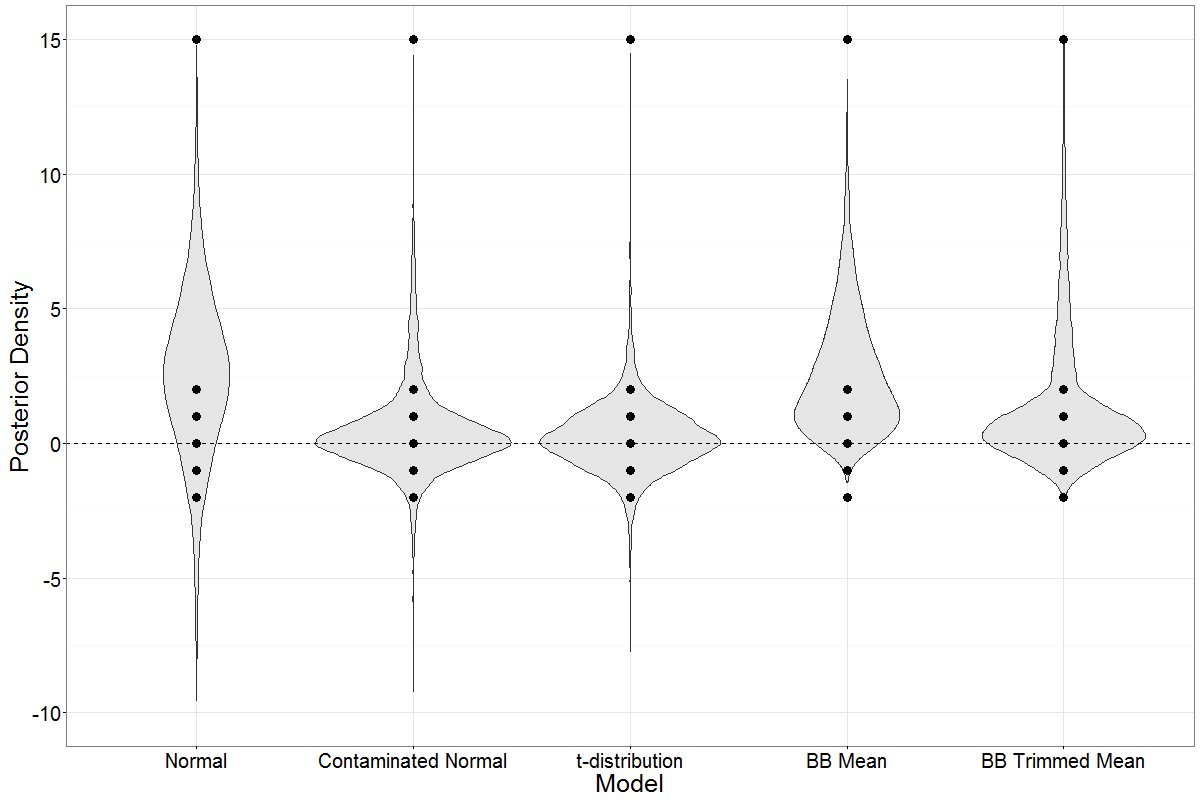
\includegraphics[width=14cm]{violins.png}
    \caption{Posterior distributions for the population mean (or trimmed mean) when given a small data set containing one outlier, according to the       different approaches.   The dotted line represents the true population mean (without the contaminated point). If the model is estimating the mean well, we would hope the posterior to be peaked near or on the mean.   The normal model (leftmost plot) is strongly influenced by the outlier. To a lesser extent, so is the Bayesian bootstrap interval for the mean (    fourth   plot from the left). The contaminated normal model (second from the left)  , the t-distribution model (middle),   and the Bayesian bootstrap interval for the trimmed mean (rightmost plot) are all less sensitive to the extreme data point.}
    \label{violins}
\end{figure}

Armed with     five   Bayesian models, we first consider a problem familiar to anyone who has taken an undergraduate research methods class. Suppose a particular experimental condition yields the following six observations:\footnote{  These numbers were arbitrary, but interestingly enough are also used in the toy example given in \textcite[][Figure 16.5, p. 460]{kruschke2014doing}.}
$$
-2,-1,0,1,2,15
$$
and the researcher wishes to construct a 95\% credible interval for the mean. It is immediately obvious that the sixth data point is an {\it outlier}, in the sense that it is quite distant from the other five. What is less than obvious is whether it also counts as a {\it contaminant}, in the sense of being an observation generated from a distribution entirely unrelated to the phenomenon of interest to the researcher. If it is indeed a contaminant it should have minimal influence on what the researcher believes about the phenomenon of interest. Noting this, it is instructive to consider what the     five   Bayesian approaches infer from these data.

The violin plots in Figure~\ref{violins} show the relevant posterior distributions for all     five   models, and it is immediately clear from inspection that the choice of model matters. According to the normal model and the BB-mean approach, the best point estimate   (calculated from the mean of the posterior)   for the population mean $\mu$ is essentially identical to the sample mean of 2.49.   The BB estimate of the population 20\% trimmed mean discounts the outlier to some extent, producing an estimate of   1.38.   The contaminated normal model   and the t-distribution model   produce       the strongest outlier discounting and estimate       a population mean of   0.47 and 0.22, respectively,   only slightly larger than the mean of the first five observations. Other inferences from these models are equally discrepant.

We next consider the the highest density intervals for the mean.\footnote{  Although all of the simulations provided in this manuscript use the highest density interval (HDI), we ran all simulations with equal-tailed intervals between the .025 and .975 quantiles. There was no qualitative difference in the results.}   According to the normal model there is a 95\% chance that the population mean lies between   $[-4.25,9.08]$   and an 18\% chance that the population mean is less than zero. The   t-distribution model and   contaminated normal model produce     much narrower 95\% credible intervals of  $[-2.23 , 2.27]$ and $[-2.49, 4.88]$ respectively,    but a much larger chance that the population mean is negative (43\% each).   A Bayesian bootstrap of the mean gives a qualitatively different interval estimate of   $[0.79 ,7.03]$,   with a lower bound noticeably closer to zero than either of the other two models. Not surprisingly, this model judges that there is only a 6\% probability that the true mean is negative. Finally, using the BB to estimate the trimmed mean produces an interval of   $[-1.60, 7.12]$   and a 27\% chance of a negative mean.

 Unique among the models, the contaminated normal model also provides an estimate of which items are contaminants: for instance, the data point 15 is given 85\% chance, while the others are identified as contaminants with less than 7\% chance. It also estimates the overall proportion of contaminants ($\gamma$ in Figure~\ref{graphicalmodels}) at 13.1\%, and the overall width of the contaminate distribution ($h$ in Figure~\ref{graphicalmodels}) as 11 times the target distribution.   As this simple example illustrates, there is   a clear difference between the performance of the t-distribution and contaminated normal models on one hand, and the other models on the other. The contaminated normal model has the added benefit of allocating the probability that each datum is an outlier.

\subsection{Systematic differences as a function of outlier extremity}

Disagreement among models is not necessarily problematic, especially when those models are provided with very few data points. In this case, however, the differences are systematic and reflect a deep incompatibility among the models. To see this, suppose we were to smoothly vary the location of the sixth data point from $x=0$ to $x=25$, and observe how the credible intervals change for all     five   approaches. The results are shown in Figure~\ref{toyproblem}, and reveal fundamental differences in how the models behave.

For the normal model and the BB-mean approach, the best estimate of the population mean tracks the sample mean: the more extreme the outlier becomes, the more extreme the estimated population mean comes. In contrast,   the t-distribution model,   contaminated normal and BB-trimmed methods       all discount the outlier but  do so in qualitatively different ways. The BB-trimmed method discounts the most extreme observations, but the extent of the discounting does not depend on the magnitude of the extremity: the estimated population mean rises more slowly than the sample mean, but it rises monotonically. Making the outlier more extreme {\it always} increases the estimated population mean.

The contaminated normal model shows a fundamentally different pattern. For very modest outliers (up to about $x=6$) the contaminated model behaves in a similar fashion to the normal model and the BB-mean approach, and the estimated population mean is almost identical to the sample mean. Above this point, the contaminant model begins to discount the outlier, reducing its influence on the estimated population mean. Eventually a point is reached that the model becomes so certain that the outlier is a true contaminant that any further increases to the outlier act to {\it reduce} the estimated population mean. By the time that the outlier reaches $x=25$ the model has discounted it almost completely, and the estimated population mean falls back towards zero (the mean of the other five observations). This pattern is fundamentally at odds with the one produced by the BB-trimmed method.

The t-distribution model performs differently again.  Much earlier than the contaminated normal model (i.e. before the outlier has reached a value of 5), it begins to  discount this extreme point, producing a credible interval that is relatively consistent regardless of the value of the outlier.


\begin{figure}[p]
    \centering
    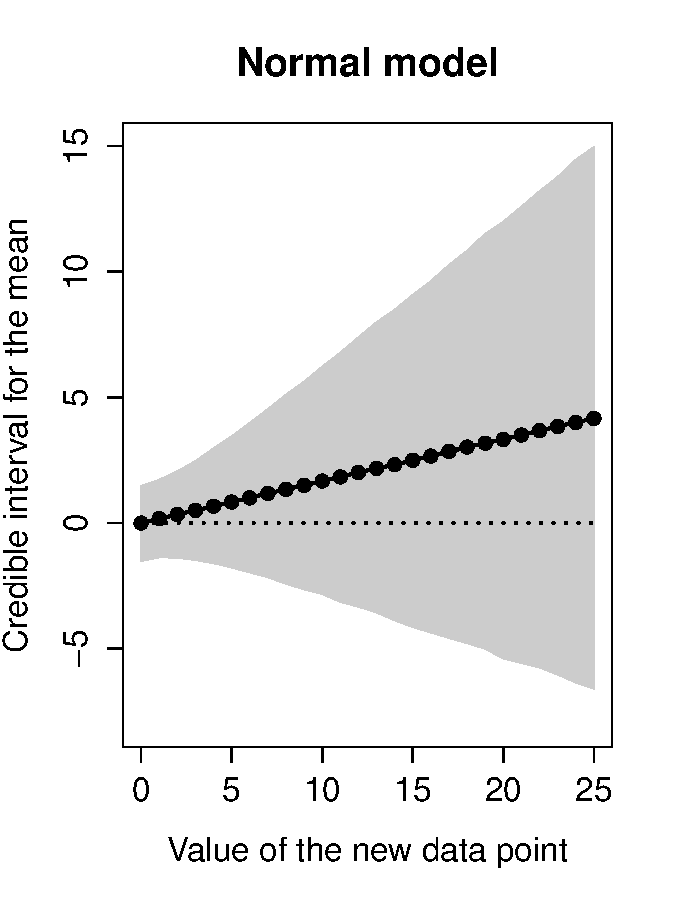
\includegraphics[width=5.0cm]{CI_n.pdf}
    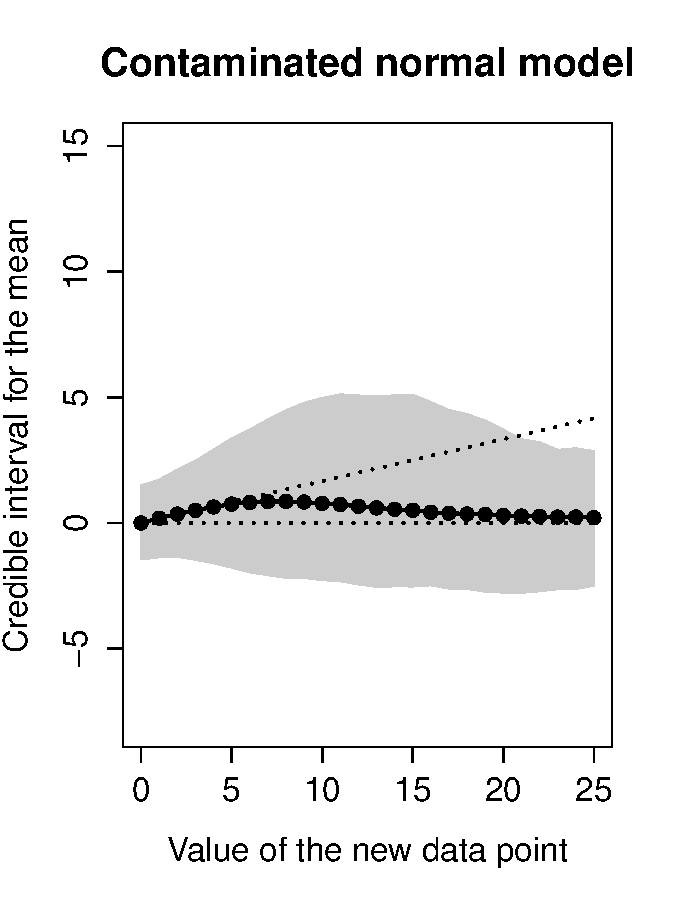
\includegraphics[width=5.0cm]{CI_cn.pdf}
    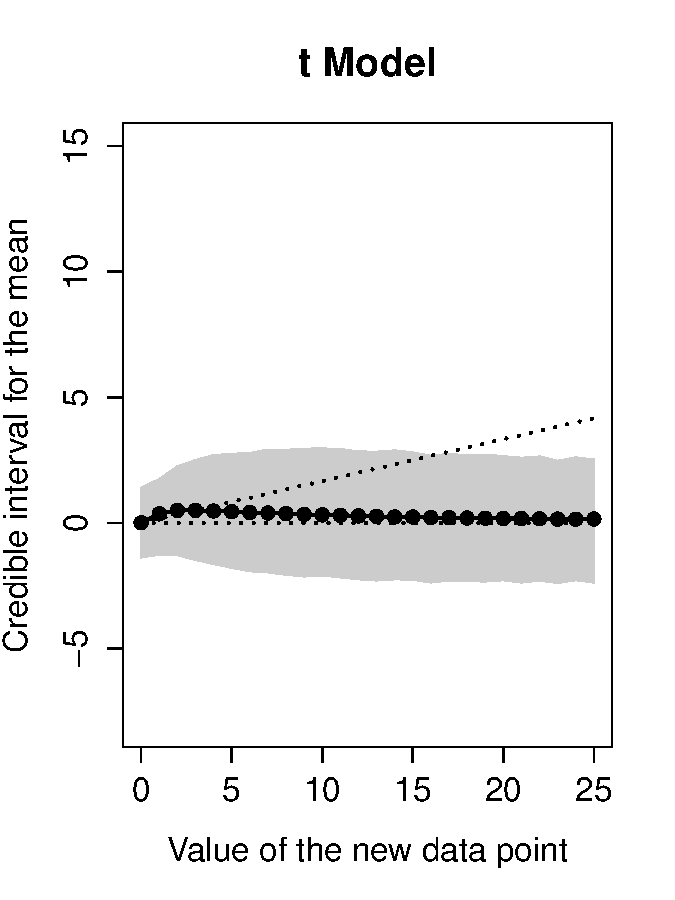
\includegraphics[width=5.0cm]{CI_tModel.pdf}
    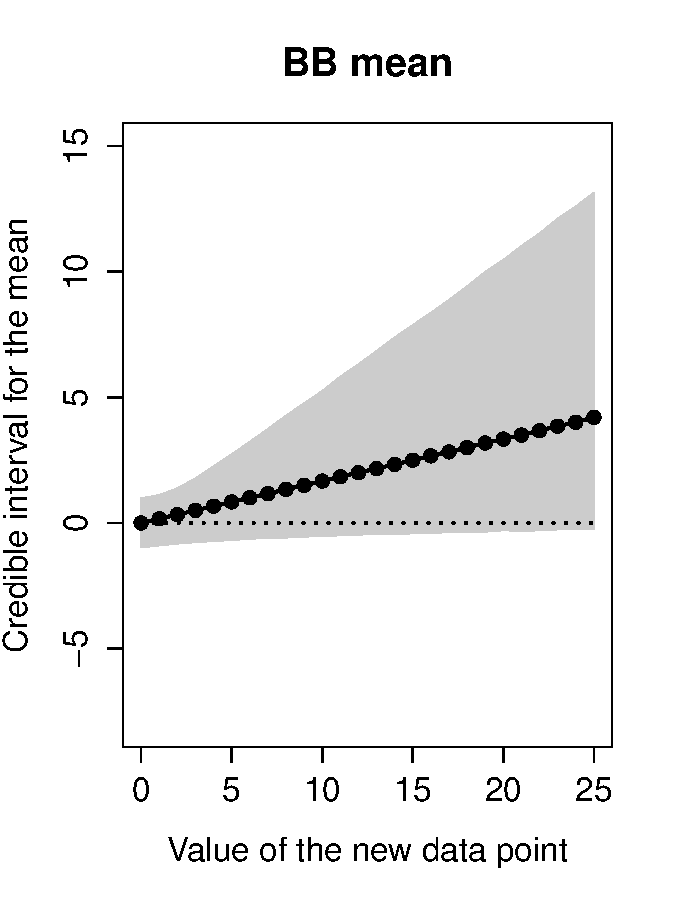
\includegraphics[width=5.0cm]{CI_bbm.pdf}
    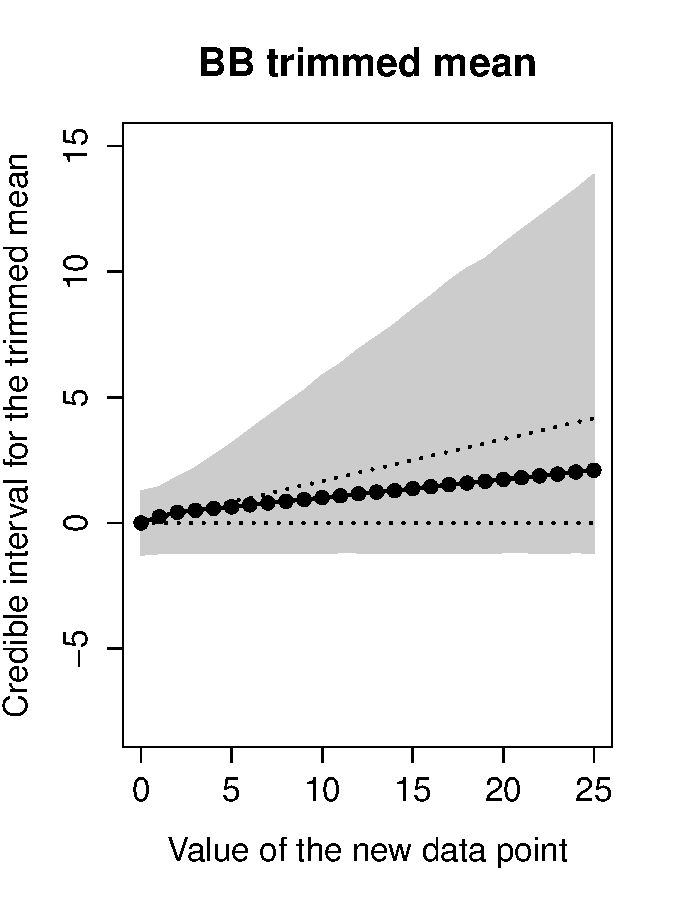
\includegraphics[width=5.0cm]{CI_bbtm.pdf}
    \caption{An illustration of how the credible intervals change as a function of the extremity of an outlier. Each observed sample contains the values $-2$, $-1$, $0$, $1$ and $2$ in equal proportions. The y-axis represents the width of the credible interval for these points plus a contaminant. The values on the x-axis represent the extremity of the contaminant point. As these values increase, the distance between this point and the rest of the sample grows.   The dark points show the population mean estimated by the model for each value of contamination. The light grey points show the mean of the sample distribution both with and without the extreme point.   The normal, BB mean and BB trimmed produce intervals that increase monotonically as the outlier grows more severe. Conversely, the contaminated normal model does not. Once an outlier is sufficiently extreme, the model discounts it and produces a credible interval on the remaining sample.   The t-distribution model discounts the moderately small outliers to the same degree as the extremely large outliers.   }
    \label{toyproblem}
\end{figure}

\begin{table}[p]
\caption{  Qualitative differences among the five different Bayesian approaches are summarized here. This table is a summary of the findings demonstrated in Figure~\ref{toyproblem}, and summarises the theoretical expectations of how the models incorporate the outlier and thus how the beliefs about the mean vary across models. The third  row relates to whether the posterior (and subsequent credible interval) is symmetric around the estimate for the mean. The last row addresses how the outliers are treated by the model.}
\label{qualitativediffs}
\vspace*{6pt}
\begin{tabular}{p{6cm}|p{1.5cm} p{1.5cm} p{1.5cm} p{1.5cm} p{1.5cm}}\small
& Normal & Contam-inated & t-dist& BB-mean & BB-trimmed \\ \hline
Should outliers be discounted when estimating means? & No & Yes & Yes & No & Yes \\
Do beliefs about the mean reverse as the outlier becomes very extreme? & No & Yes & No & No & No \\
Should uncertainty at the upper end be mirrored in the lower end? & Yes & Maybe & Yes & No & No \\
Does the model allow explicit outlier labelling? & No & Yes & No & No & No
\end{tabular}
\end{table}



A similarly dramatic disagreement appears when we consider how the credible intervals change. The normal distribution   and  t-distribution models are     symmetric, and as a consequence any increase of uncertainty at the upper end of the interval must be mirrored by increasing the uncertainty at the lower end as well. The nonparametric model that underpins the BB imposes no such symmetry constraint, and so the upper and lower tails of the credible interval move relatively independently. For both BB models a shift in the outlier produces a change in the upper end of the credible interval that matches the change produced by the normal model, but the lower bound is largely unaffected.

The contaminated model produces a different pattern again. For relatively modest outliers (again, up to about $x=6$) the upper and lower bounds of the interval look essentially identical to the normal model, and satisfy the same symmetry constraints. However, once the model begins to discount the outlier a different pattern emerges. The lower bound to the credible interval stays roughly constant, not too dissimilar to the nonparametric models. The upper bound, continues to rise for a while but eventually it too begins to fall back down as the model becomes increasingly certain that the outlier is a contaminant.

The various disagreements among models are summarized in Table~\ref{qualitativediffs}, which characterises the differences in terms of three questions about how credible intervals should behave and how beliefs should change as a function of the extremity of an outlier. As the table highlights, the differences are not simple differences of opinion about priors (e.g., how big an effect size is expected); they are fundamental questions about the relationship between data and beliefs. In our view at least, the behavior of the contaminated normal model most closely matches what we think most (but not all) scientists would consider reasonable in most (but not all) psychological experiments. To the extent that this is true, a contaminated normal model makes considerably more sense as a default choice for the analysis of behavioral data.


\subsection{Increasing the sample size does not erase the differences}

A different perspective on the same issue is to consider how the models make different inferences as a function of sample size. In real data analysis problems, adding new data also changes the distribution of those observations. For the purposes of illustrating the ``pure'' effect of sample size, we create a sequence of data sets by adding multiple copies of the same six values $X=(-2,-1,0,1,2,15)$, and apply all     five   methods to the data. The results are shown in Figure~\ref{toyproblem2}.

Unsurprisingly, as the sample size increases, the normal model and the BB mean approach continue to produce estimates of the population mean that track the sample mean of 2.5, and the credible intervals tighten around that mean. Equally unsurprisingly, as the sample size increases the BB estimate of the 20\% trimmed population mean  converges to the 20\% trimmed mean of the observed data, yielding a value of 0.5 in the large sample limit. The contaminated normal model   and t-distribution model   produce      a different answer again: as the sample size increases the model s   become     increasingly certain that the outliers (the copies of the $x=15$ observations) are contaminants, and       converge      to the mean of the other observations, yielding an estimated population mean of 0.   The contaminated normal model, whilst producing a wider credible interval for small $n$, produces  a slightly tighter credible interval than the t-distribution model as $n$ grows large.

\begin{figure}[p]
    \centering
    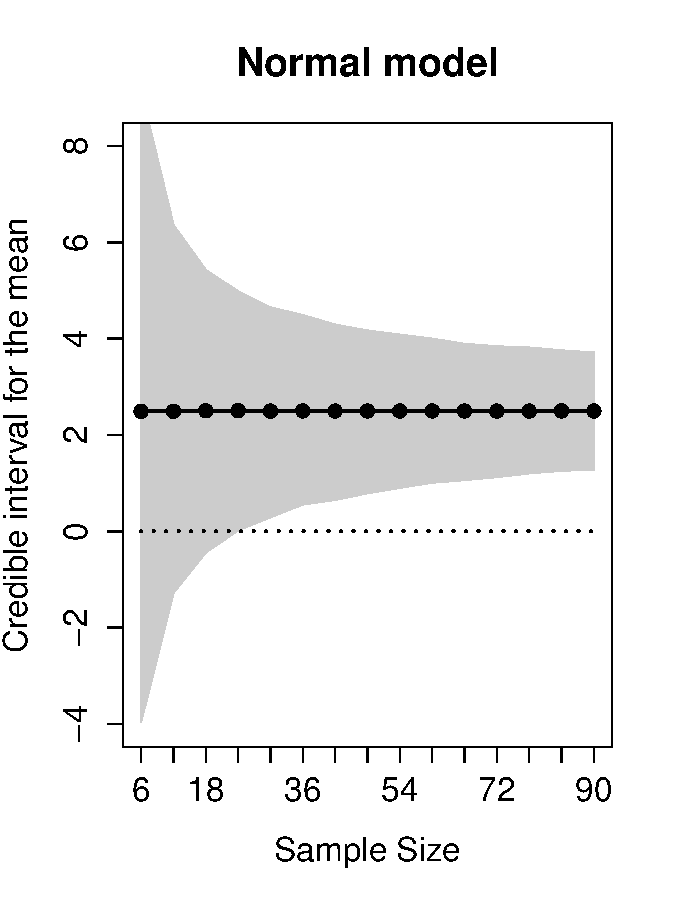
\includegraphics[width=5.0cm]{CI2_n.pdf}
    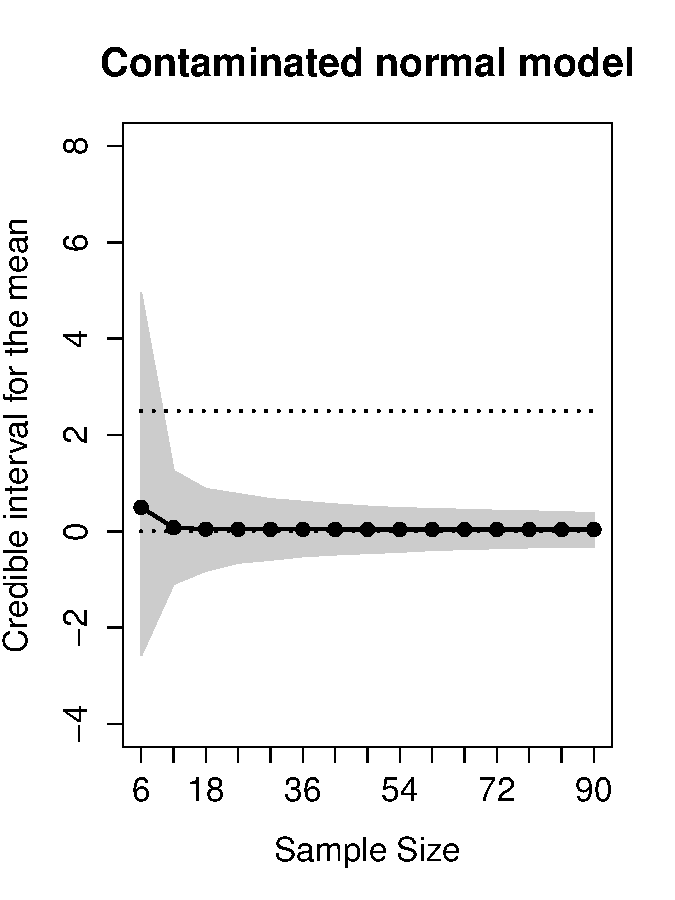
\includegraphics[width=5.0cm]{CI2_cn.pdf}
    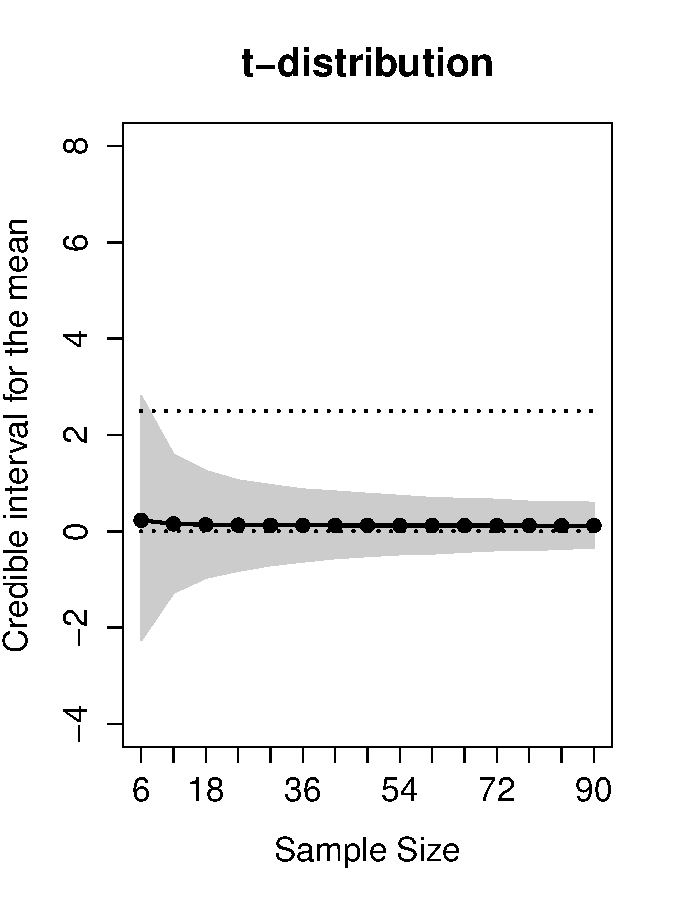
\includegraphics[width=5.0cm]{CI2_tModel.pdf}
    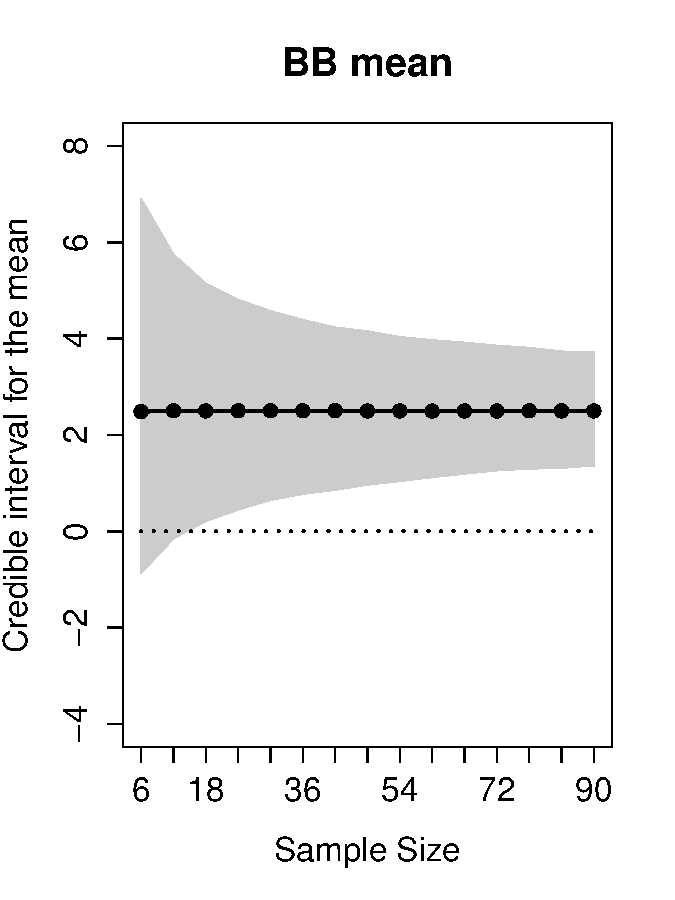
\includegraphics[width=5.0cm]{CI2_bbm.pdf}
    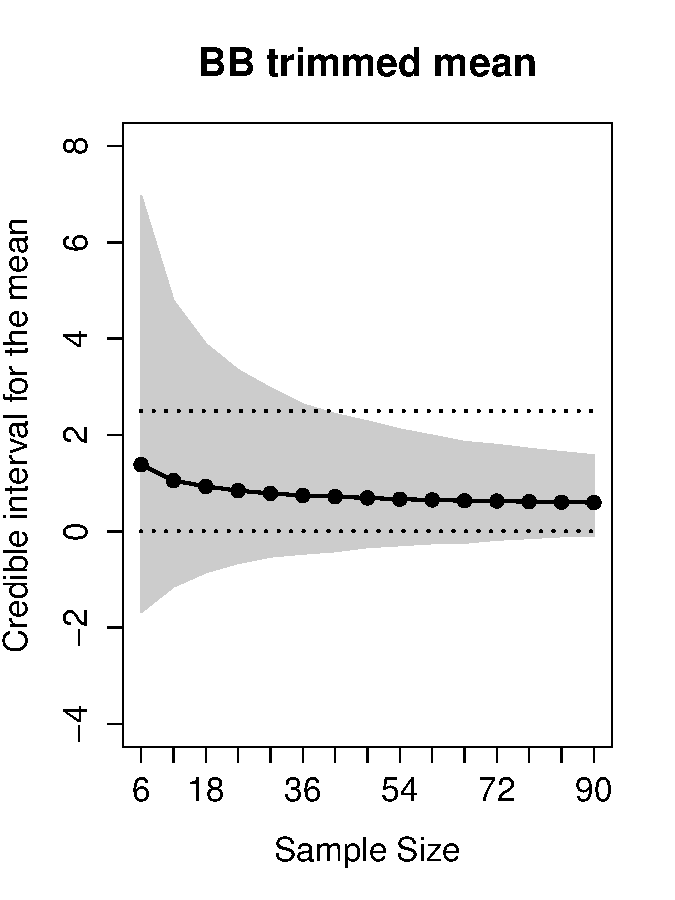
\includegraphics[width=5.0cm]{CI2_bbtm.pdf}
    \caption{An illustration of how the credible intervals change as a function of sample size. To control for the effect of distribution, at every sample size $n$ the observed sample contains the values $-2$, $-1$, $0$, $1$, $2$ and $15$ in equal proportions. The y-axis represents the width of the credible interval. The x-axis represents the sample size.   As before in Figure~\ref{toyproblem}, the  dark points show the population mean estimated by the model for each value of contamination. The light grey points show the mean of the sample distribution both with and without the extreme point.   The convergence rate of the normal model, BB mean and BB trimmed models are roughly similar, whilst the contaminated normal model converges much faster. The normal and BB mean models converge to approximately 2.5, the BB trimmed mean converges close to 0, and the contaminated normal model   and t-distribution models converge   to approximately 0.}
    \label{toyproblem2}
\end{figure}

To a statistician, none of these results might seem especially surprising: models that rely on different assumptions can produce quite different estimates of the same (or similar) quantity. To an empirical scientist, they might be somewhat problematic. The fact that the differences between models can be exaggerated by collecting additional data has non-trivial implications. It is not possible to avoid the problem of contaminants simply by being Bayesian, nor is it possible to sidestep the issue simply by collecting more data. To resolve the problems that these incompatibilities pose, substantive choices must be made by the data analyst.


\subsection{How robust are the different methods?}

The examples in the previous section highlight the importance of taking contamination seriously. In order to provide a better picture of how each of the     five   methods performs, we present a simulation study that investigates the behavior of different Bayesian models when contaminants are introduced to the data. We consider two qualitatively different kinds of contamination, {\it biased contamination} and {\it unbiased contamination}, depicted in Figure~\ref{contaminanttypes}. In both instances we assume that there exists a target population distribution (shaded plot) that represents the phenomenon of substantive interest to the researcher, but the data set is corrupted: some proportion of the data arise from a contaminant distribution (grey plot) that is of little substantive interest.

The unbiased contamination scenario exactly matches the assumptions that underpin the contaminated normal model: the mean of the contaminant distribution is the same as the mean of the target distribution, but it has higher variance. In contrast, a biased contamination scenario is one in which the contaminants arise from a distribution that has a different mean from the target, and is potentially more worrisome.\footnote{In these simulations we assume that the contaminants are normal. We also ran a version in which the contaminants were generated from a clumpy distribution, which we did by sampling contaminant distributions from a Dirichlet process. However, apart from making the results somewhat more variable everywhere, we did not find that clumpy contamination made much of a difference to our simulation results, and as such we have restricted our discussion to the case when contaminants are normally distributed.} Specifically, in our simulations the target distribution was always assumed to be a normal distribution with mean 0 and standard deviation 1. Unbiased contaminants were sampled from a normal distribution with mean 0 and standard deviation 10, whereas biased contaminants were sampled from a normal distribution with mean 10 and standard deviation 1.

\begin{figure}[t]
\centering
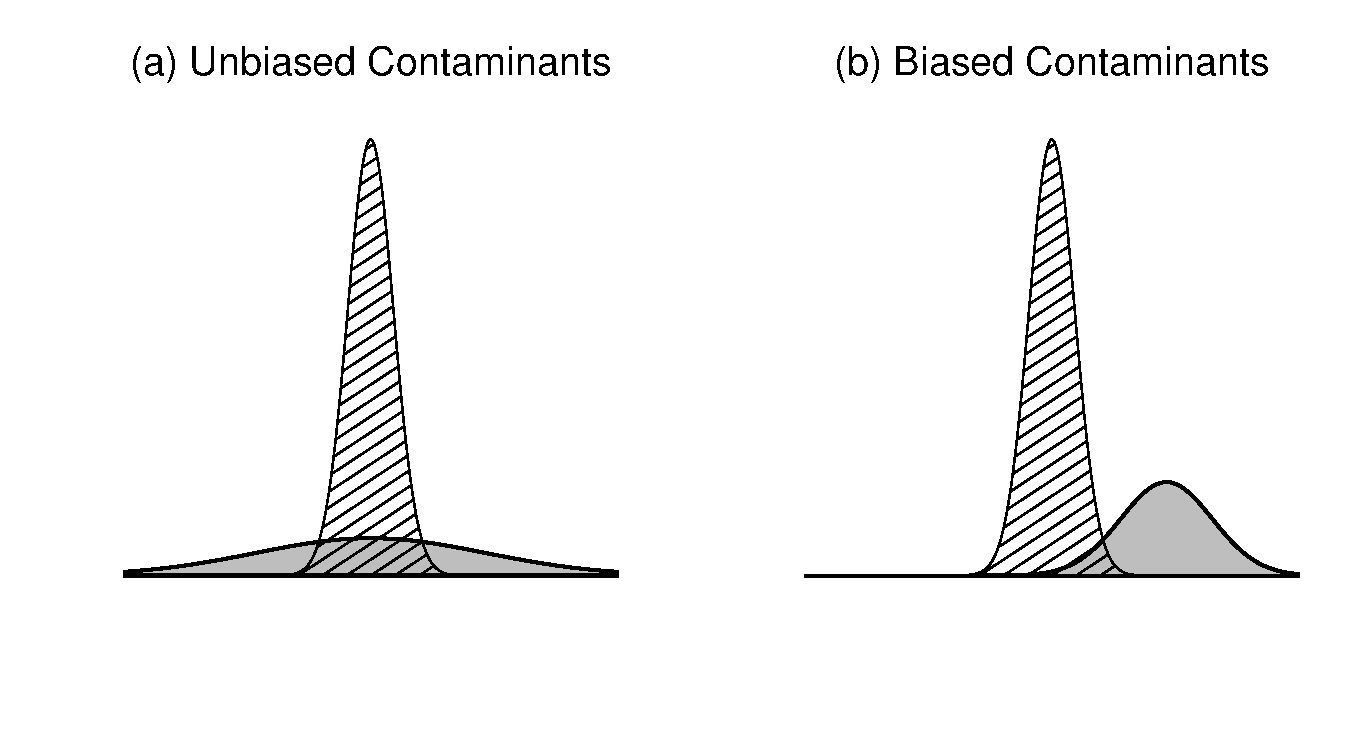
\includegraphics[width=10cm]{contaminantTypes.pdf}
\caption{Two qualitatively different kinds of contaminant distribution. Each panel plots a target distribution (shaded) mixed together with a contaminant distribution (grey). In the {\it unbiased contamination} scenario (panel a) the contaminants are generated from a normal distribution that has high variance but is centred on the same location as the target distribution. In the {\it biased contamination} scenario (panel b) the contaminants have a different mean to the target distribution.}
\label{contaminanttypes}
\end{figure}


In addition to varying the {\it kind} of contamination, we varied the {\it amount} of contamination from 0\% to 50\%. In practice we would expect that the proportion of contaminants should be well below 50\% -- indeed, if half of one's data are ``contaminants'' it does not seem to make sense to consider them contaminants any more. As mentioned earlier in the paper we expect that a value of 10\% is more reasonable, but given that our focus is developing statistical methods that are robust even in somewhat extreme situations, it seems sensible to consider the full range of possibilities. Finally, we varied the sample size, considering values with $N=20$, $50$, $100$ and $250$ in order to cover the range of typical sample sizes in behavioral research. For each scenario we ran 1000 random simulations.


\begin{figure}[p]
\centering
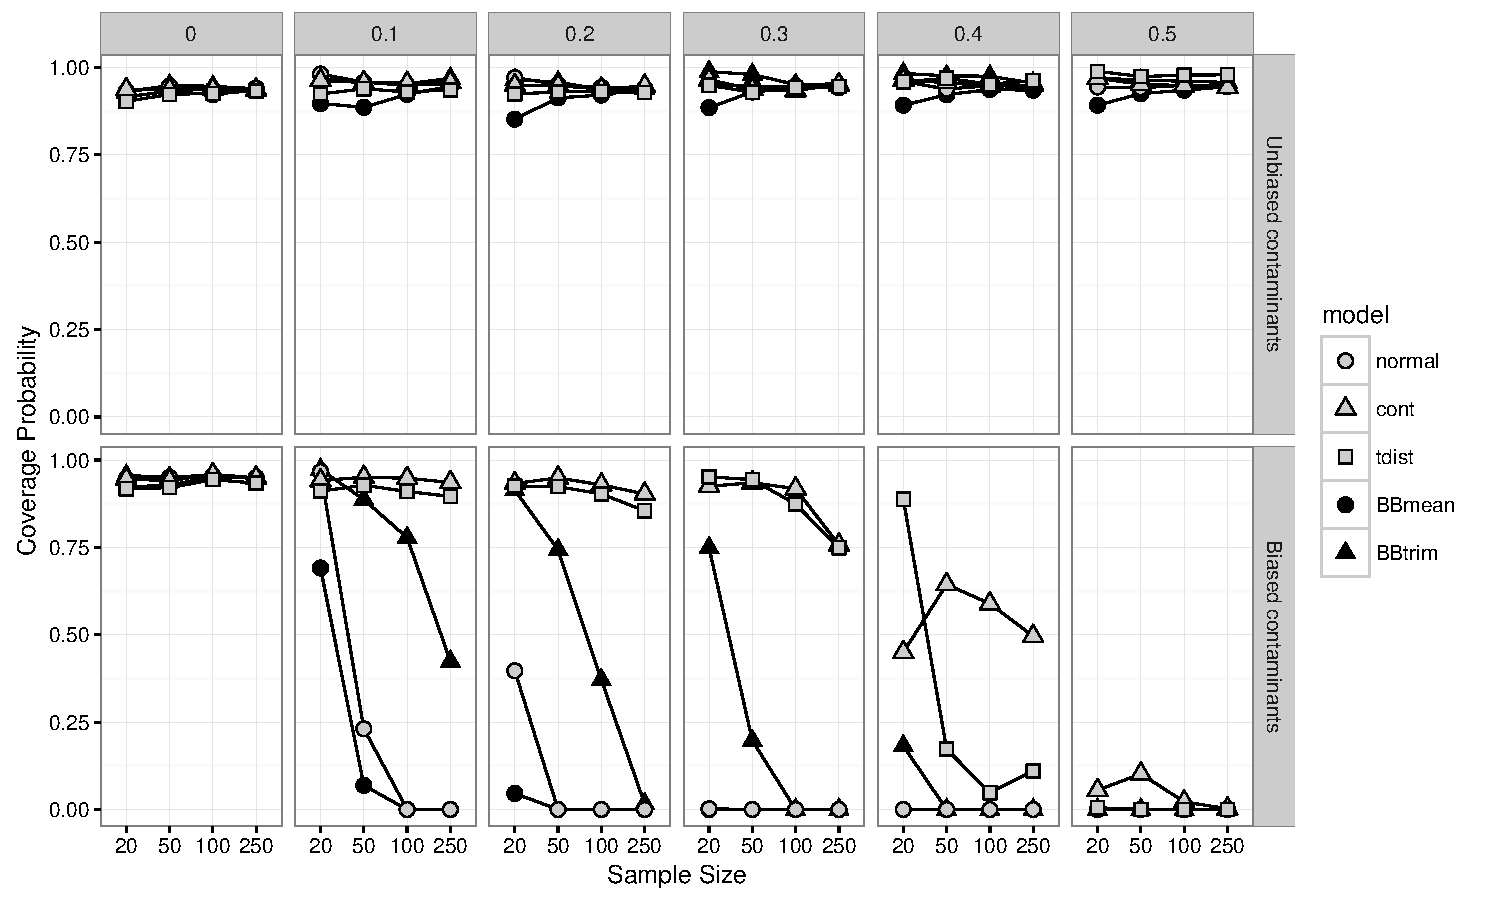
\includegraphics[width=14cm]{simCover.pdf}
\caption{Coverage probability (proportion of cases in which the interval contains the true mean) for all five Bayesian methods as a function of sample size (x-axis), contaminant proportion (horizontal panels) and contaminant type (vertical panels). Insofar as each of these represents a 95\% credible interval, ideally one hopes to see 95\% coverage. Except for the BB mean, all of the models have good coverage probability when the contaminants are not biased to one side of the sample. As expected, when the contaminants are biased, all of the models eventually fail with 50\% contamination, even with a very large sample. The contaminated normal model however, is robust at a much higher level of contamination (40\%)   than   even the t-distribution.    }
\label{simcover}
\end{figure}

\begin{figure}[p]
\centering
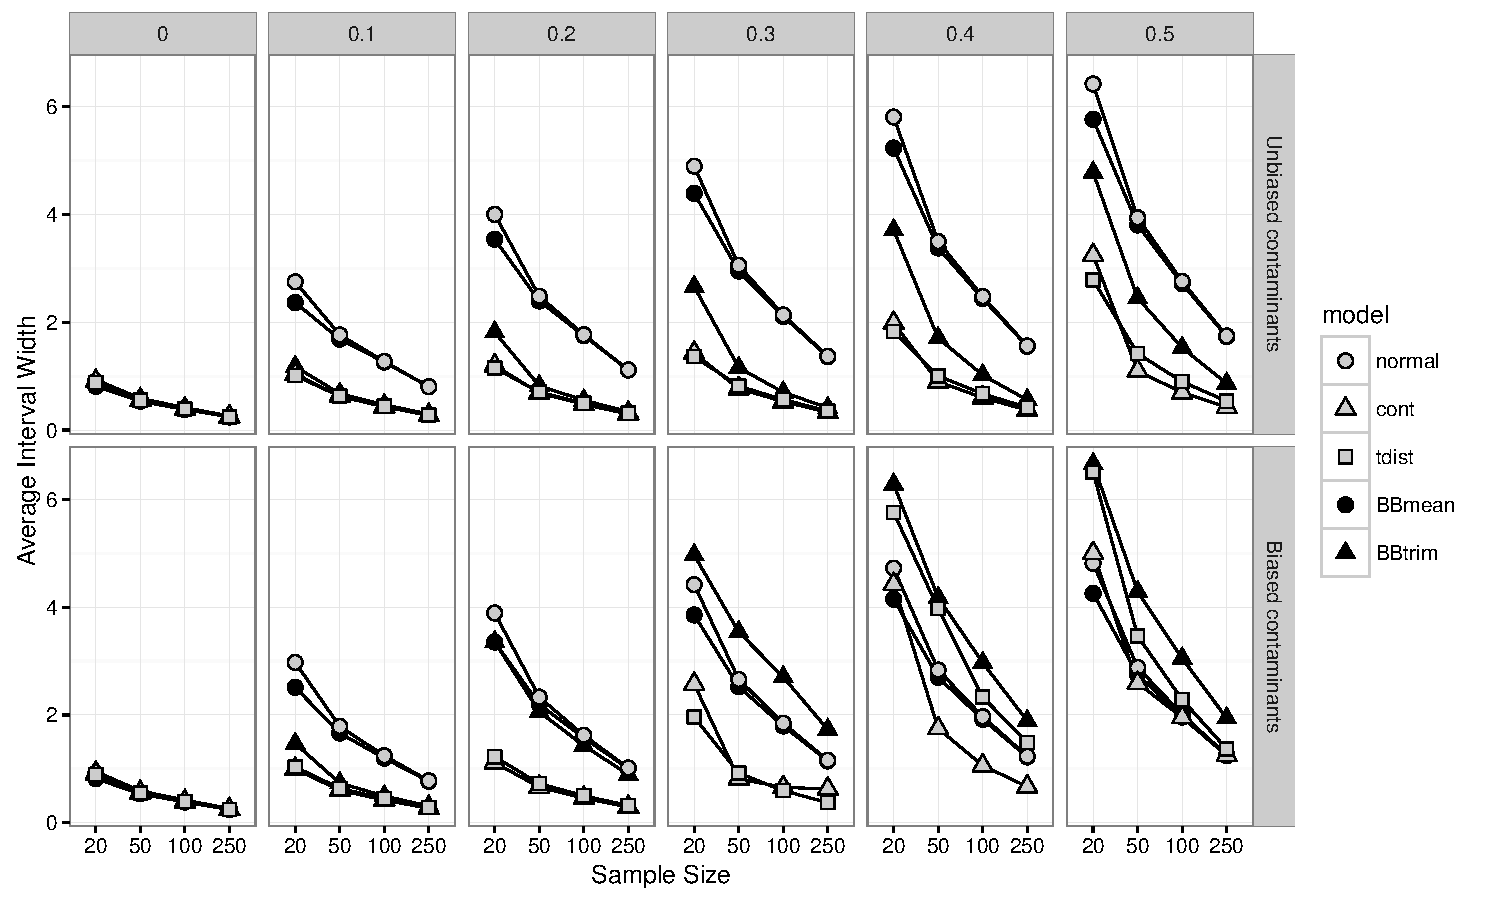
\includegraphics[width=14cm]{simWidth.pdf}
\caption{Average interval width (y-axis) for all four Bayesian methods as a function of sample size (x-axis), contaminant proportion (horizontal panels) and contaminant type (vertical panels). Although some contaminants produce wider intervals than others, they are quite similar in size. This suggests that the robustness in Figure~\ref{simcover} is not an artifact of more conservative (wider) credible intervals.}
\label{simwidth}
\end{figure}

The results are plotted in Figures~\ref{simcover} and \ref{simwidth}. In the top row of Figure~\ref{simcover} we see that when the contaminants are unbiased, all four Bayesian methods have reasonable coverage -- in the frequentist sense of trapping the true mean with the desired 95\% probability\footnote{We have on occasion encountered Bayesian data analysts who oppose any evaluation of the frequentist properties of Bayesian methods, arguing that Bayesian methods should be defined on their own terms with no reference to frequentist concepts such as consistency, efficiency, unbiasedness etc. We can understand this impulse, but we take a pragmatic view ourselves. To the extent that these simulations annoy a truly committed Bayesian, we propose that even a committed Bayesian is entitled to treat the entire frequentist apparatus as an elaborate elicitation study: if a model produces long run behavior that the data analyst does not find desirable, it must be the case that this is not a model that the analyst places any (subjective) belief in. In that sense a frequentist evaluation can be very useful to a Bayesian researcher, as a method for uncovering revealed preferences.} -- for most choices of sample size and contamination level, suggesting that for the most part these methods are robust when contaminants are unbiased. The one exception to this is the BB mean approach (plotted with black triangles), which performs noticeably worse than the other three approaches when the sample size is small and the contamination level is low. The reason for this is that small sample sizes and lower contamination rates is exactly the situation in which it is most likely for all the contaminants to lie on the same side,  thereby producing data that is more representative of the biased    contaminant   situation, and (as we discuss below), the BB mean model does not fare well when faced with biased contamination.

In addition to measuring the coverage probability for the different estimators, we also examined the precision (i.e., average width) of the credible intervals produced be each of the four methods. The top row of Figure~\ref{simwidth} suggests that the average width of the credible intervals does not differ greatly among all four methods. Taken together with the results in Figure~\ref{simcover} the simulations suggest that unbiased contaminants are comparatively harmless, having only modest influence on the accuracy or size of the credible intervals. To the extent that contaminants are unbiased, one might reasonably conclude that Bayesian inference using the default normal model is genuinely robust, and there would be little need to consider alternative approaches.

When we turn our attention to the case when the contaminants are genuinely biased, a different story emerges. As the bottom row of plots in Figure~\ref{simcover} the normal model and the BB estimate of the mean are both very sensitive to biased contaminants: even a modest level of contamination (e.g., 10 contaminants in a sample of 100 observations) is enough to make it virtually certain that 95\% credible intervals constructed using these methods does not contain the mean of the target distribution. The failure of the BB mean approach is particularly noteworthy because it highlights   that, like the frequentest bootstrap,   nonparametric approaches are not automatically robust: using the Bayesian bootstrap to estimate the posterior distribution for the parameter mean frees the researcher from the assumption that the population is normal, but it does not provide any mechanism to identify or exclude contaminants. As such, when the contaminants are biased, so too is the the BB estimate of the population mean.

The other     three   methods perform rather better. The BB estimate of the population 20\% trimmed mean is somewhat improved, but -- somewhat unsurprisingly -- it too becomes unreliable once the proportion of contaminants rises above the trimming level: at 30\% contamination it is only marginally better than the other two methods. The contaminated normal model   and t-distribution model,   on the other hand, are both extremely robust,   performing similarly to each other up to 30\% contamination level.    At a massive 40\% contamination, the contaminated normal model produces a   credible interval   that   contains the true mean in more than 50\% of cases, beaten by the t-model only in the smallest sample size.

Again we note a slight inconsistency. With higher contamination levels (greater than 40\%) the contaminated normal model produces a curious result. Unlike the other models (which start at their most accurate and decrease with increased $n$), the contaminated normal model is less     likely   to contain the true mean with 20 samples than 50 samples. This is because the contaminated normal model estimates the contaminant proportion using information from both the prior (which assigns a very small probability to such high levels of contamination) and the data observed. With very small sample sizes, the data provide very  little evidence to suggest a high level of contamination. As such the model relies more heavily on the prior and incorrectly identifies contaminated points as members of the target distribution (e.g., only $29\%$ of contaminants are correctly identified at a $40\%$ contaminant level with $N=20$). However, unlike the other models, increasing the sample size does lead to better estimation of the contaminant proportion (i.e. an increase to $70\%$ correctly identified at $40\%$ contaminant and $N=50$). This increases the chance of creating a credible interval that contains the true mean.

Finally, we turn our attention away from the coverage probability and consider the precision (as measured by width) of the intervals in the biased contaminant scenario.     Consistent   with our earlier findings in the unbiased scenario, the robustness of the contaminated normal model does not seem to come at the expense of precision. As the bottom row of Figure~\ref{simwidth} shows, the credible intervals produced by the contaminated normal model tend to be as narrow as those produced by the other approaches. It is noteworthy that the width of the intervals produced by contaminated normal model decreases with increased sample size in much the same manner as the other models. This suggests that the increased robustness of this model is not an artifact of the model producing more conservative (i.e. wider) intervals.


\section{  Detecting contaminants in the data}

In this manuscript we considered five different methods of creating a credible interval for the mean. Overwhelmingly the contaminated normal model and t-distribution model perform best when contamination is present. However, they employ very different methods of accounting for this contamination. The t-distribution model accounts for outliers because its tails can be heavier than the tails of a normal distribution. The contaminated normal model, by contrast, is a mixture model of a target distribution and a (much wider) contaminant distribution. Because it is a mixture model, every datum has some probability of being in the contaminant distribution. No other model that we have described in this paper has this feature.

We have argued that this feature is rather desirable for a number of reasons. To more fully demonstrate the main one -- that it identifies which specific data points are likely to be the outliers -- we repeat the simulations from Figure~\ref{toyproblem}, but now investigate the probability that the extreme point is identified as an outlier. As Figure~\ref{cont_prob} shows, the contaminated normal does well at outlier identification. Initially the extreme point is included in the target distribution, but as that point grows large relative to the rest of data it is increasingly categorized as part of the contaminant. This mirrors the shape of the credible interval in Figure~\ref{toyproblem}.

\begin{figure}[p]
    \centering
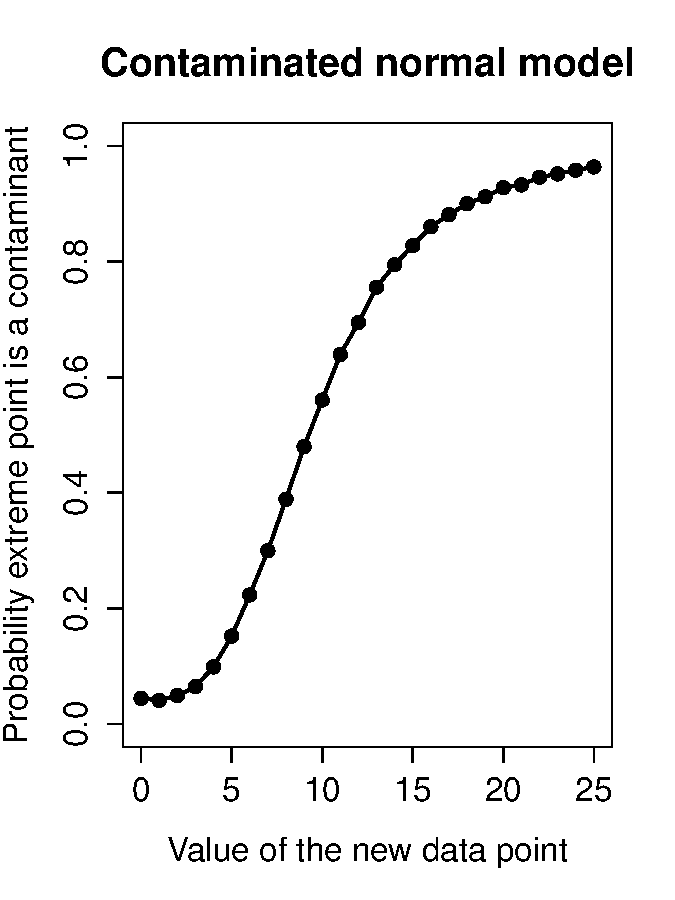
\includegraphics[width=5.0cm]{toyContRejection_cn.pdf}
    \caption{  An illustration of the probability of the extreme point being labelled as an outlier by the contaminated normal model. The values on the x-axis represent the extremity of the contaminant point. The y-axis represents the probability of this point being classified as a contaminant relative to the other data.
    As the value grows more extreme, it becomes much more likely to be rejected as a contaminant.  }
    \label{cont_prob}
\end{figure}


\section{Discussion}

Statistical inference necessarily relies on simplifying assumptions: the causal mechanisms that produce empirical data are usually complicated, and researchers typically do not understand the phenomenon under investigation well enough to properly specify what those mechanisms are (or else why would one be studying it?). The truism that ``all models are wrong'' is an expression of this necessity \parencite{box_science_1976}. However, the fact that all models are wrong does not imply that all simplifying assumptions are equally sensible. Given the inherent difficulties associated with behavioral research, we argue that if a data analysis tool is intended to serve as a ``default'' method for behavioral researchers, it must be robust in the face of contaminated data. In practice is difficult to trust the inferences produced by a statistical model if that model is extremely sensitive to contaminants. This point is acknowleged within the orthodox literature on robust statistics \parencite{wilcox_introduction_2012}, but has received comparatively little attention within Bayesian behavioral statistics.\footnote{We do not suggest that Bayesians are unaware of this as an issue (see \textcite{wang_general_2015} for example), merely that research has tended to focus on different questions.}

In this paper we restricted ourselves to a very simple statistical problem -- the estimation of a credible interval for the population mean of a continuous univariate quantity -- and to a set of     five   Bayesian approaches that are by no means exhaustive, but are arguably representative of the class of models that researchers might consider applying. In some respects our findings would not surprise any statistician: the default normal model is not robust to contamination, and a nonparametric approach is not necessarily better if applied in a naive way. The Bayesian bootstrap approach {\it is} somewhat robust if it is used to construct credible intervals for a quantity (population trimmed mean) that is not easily influenced by the tails of the distribution, but it is not at all robust when it is directly applied to estimate the population mean itself. This finding is mirrored in the parametric models as well: although we find that the default normal model is not robust, the   t-distribution model and   contaminated normal model     are   very robust, and appear to remain robust even when   \sout{(as per the biased contamination scenario)}   the contamination process violates the underlying assumptions of the model.  At very high levels of contamination the t-distribution model is not quite as robust as the contaminated normal model and also provides no indication about which items are most likely to be outliers.

In view of the fact that Bayesian methods are not robust to contamination simply by virtue of being Bayesian, to the extent that contamination is commonplace in behavioral research, it seems sensible to prefer those models that are robust to contamination. We suggest that the contaminated normal model,   the t-distribution,   and the Bayesian bootstrap approach for inference about trimmed means all meet this criterion. In our simulation studies, the contaminated normal model seemed to perform     best,   but some caution is warranted since the relative robustness of these     three   methods almost certainly depends on the situation. When the population distribution is skewed, for instance, one might expect the contaminated normal model to perform poorly relative to the BB-trimmed method.  More generally, when choosing among different approaches that have some claim to being labelled ``robust'', we suggest that the qualitative considerations listed in Table~\ref{qualitativediffs} provide a better guide to researchers than relying too heavily on any one simulation study. Our personal view is that in most situations the behavior of the contaminated model is the closest match to what a human reasoner would consider sensible, but ultimately the choice of model has to depend on the context.

  That said, one advantage of Bayesian methods in general is that they make it easy to implement multiple ways to model data with outliers, some but not all of which we evaluated here. For instance, t-distributions can be straightforwardly implemented in JAGS and Stan, along with contaminant models for logistic regression and other hypothesis testing models. The textbook {\it Doing Bayesian Data Analysis} \parencite{kruschke2014doing} is an accessible resource for many such approaches.


Finally, it is worth commenting on the generality of the problem under consideration. On the one hand, this paper does focus on a very simple problem. On the other hand, the problem is one faced by almost every paper reporting empirical data: in many areas of psychology and other behavioral sciences it is standard to report  interval estimates for the population mean in various experimental conditions, and it is exactly this situation that we have considered. That being said, a natural extension of the work is to move beyond estimation problems to hypothesis testing scenarios. The contaminated normal model represents a sensible and simple tool for robust Bayesian estimation, and it is naturally extensible to construct robust Bayesian t-tests, ANOVAs and regression analyses. We are currently working on exactly these extensions.

  In addition, although this paper is focused on data analysis, very similar problems arise for human learners in the real world. The data available to people is often contaminated with outliers of one sort or another, and a robust learner would need to deal with them just as statisticians do. The mixture model we employ here may be appropriate as a cognitive model as well, and pursuing this is an interesting alternate line of research.   In the meantime, however, it seems clear -- even on the basis of this initial investigation -- that   for a statistician   the issue of robustness is just as   critical for evaluating   Bayesian models as it is for orthodox approaches, and should be given consideration when choosing the appropriate data analysis tool.



\printbibliography


\end{document}
